\documentclass[11pt]{article}
\pdftrailerid{}
\usepackage[T1]{fontenc}
\usepackage[utf8]{inputenc}
\usepackage{lmodern}
\usepackage[margin=1in]{geometry}
\usepackage{amsmath,amssymb,amsthm,mathtools}
\usepackage{booktabs,enumitem,microtype}
\usepackage{xcolor}
\usepackage{tikz}
\usetikzlibrary{arrows.meta,positioning}
\usepackage[hyphens]{url}
\usepackage[colorlinks=true,linkcolor=blue!45!black,citecolor=blue!45!black,urlcolor=blue!45!black]{hyperref}
\hypersetup{pdftitle={Uniform computation of the squared-logarithmic k-server bound},pdfauthor={OpenAI}}
\AddToHook{cmd/thebibliography/after}{\addcontentsline{toc}{section}{\refname}}
\newcommand{\E}{\mathbb E}
\newcommand{\NN}{\mathbb N}
\newcommand{\QQ}{\mathbb Q}
\DeclareMathOperator{\OPT}{OPT}
\DeclareMathOperator{\cost}{cost}
\DeclareMathOperator{\TV}{TV}
\newtheorem{theorem}{Theorem}[section]
\newtheorem{lemma}[theorem]{Lemma}
\newtheorem{proposition}[theorem]{Proposition}
\newtheorem{corollary}[theorem]{Corollary}
\theoremstyle{definition}
\newtheorem{definition}[theorem]{Definition}
\theoremstyle{remark}
\newtheorem{remark}[theorem]{Remark}
\title{Uniform computation of the\\squared-logarithmic \(k\)-server bound}
\author{OpenAI}
\date{September 24, 2026}
\begin{document}
\maketitle
\begin{abstract}
We construct a uniform randomized \(k\)-server algorithm on finite rational
metrics with competitive ratio \(O(\log^2(k+1))\) against oblivious request
sequences. Preprocessing is polynomial in the input length, and per-request
bit complexity is polynomial in that length and the binary request-counter
length. The additive movement constant is finite and instance-dependent,
but may be enormous. The construction uses the companion squared-logarithmic
existence theorem.
\end{abstract}
\section{Introduction}\label{sec:introduction}

An online \(k\)-server algorithm maintains \(k\) labeled servers in a metric
space. Upon receiving a request, it moves one server to the requested point
and leaves the others fixed. The movement is charged according to the metric.
The offline optimum knows the entire request sequence, whereas an online
algorithm must act before seeing the next request. For an initial labeled
tuple \(s\) and a finite request word \(\sigma\), write
\(\cost_{A,s}(\sigma)\) for an algorithm's total movement and
\(\OPT_s(\sigma)\) for the minimum such cost with full knowledge of the word.
Requests are fixed independently of the algorithm's random bits, the
oblivious-adversary model. We study finite rational metrics and the bit
complexity of each online decision.

The companion theorem~\cite{SquaredLog2026} supplies a policy with
competitive ratio \(O(\log^2(k+1))\), but no procedure for computing
its decision probabilities. We ask whether this existence guarantee can
be realized by a single uniform algorithm on all finite rational metrics,
using finite computations and unbiased random bits.

\begin{theorem}\label{thm:main}
There are an absolute constant \(C\) and a polynomial \(p\) with the following
property. Let \(n\ge3\), \(2\le k<n\), let \(d\) be a rational metric on
\(X=\{1,\ldots,n\}\), and let \(s\in X^k\) be an initial labeled tuple,
with repetitions allowed. Write \(L\) for the total binary encoding length
of \(n,k,d,s\). A single uniform randomized online algorithm preprocesses
these data in at most \(p(L)\) bit operations and serves request \(r_t\),
for every reachable history and internal state, in at most
\[
 p\!\left(L+\left\lceil\log_2(t+1)\right\rceil\right)
\]
additional bit operations. It uses only unbiased random bits and moves
exactly one chosen server to each request, permitting a zero-length move.
For every fixed finite request sequence \(\sigma\) independent of those bits,
\begin{equation}\label{eq:main-bound}
 \E\cost_{A,s}(\sigma)
 \le C\bigl(\log(k+1)\bigr)^2\OPT_s(\sigma)+B_{d,k,s},
\end{equation}
where \(B_{d,k,s}\) is finite and independent of \(\sigma\) and its length.
The algorithm does not need to know that length in advance.
\end{theorem}

Here and below \(\log\) is natural, except when the base is displayed.
The worst-case bit bounds in Theorem~\ref{thm:main} imply the corresponding
conditional expected bounds. The polynomial is uniform in every input
parameter and in \(t\).

Two features of the statement are essential. First, no bound on the size of
\(B_{d,k,s}\) is imposed. Second, the permitted computation grows polynomially
with the length of the binary request counter. Our algorithm serves
requests immediately, but may serve an enormous initial number of them
using one fixed label before the constructed policy takes over. The cost
of this initial service enters \(B_{d,k,s}\). Thus polynomial preprocessing
does not imply a short delay before activation or a polynomial bound on
the additive movement loss.

\subsection{History and computational scope}

Manasse, McGeoch, and Sleator introduced the \(k\)-server problem as a metric
framework for online service problems \cite{MMS1990}. Paging is its uniform
metric case: servers represent the \(k\) pages held in a cache, and a request
to an absent page costs one move. Fiat, Karp, Luby, McGeoch, Sleator, and
Young gave the randomized marking algorithm and the harmonic randomized
lower bound for paging \cite{FKLMSY1991}. This logarithmic behavior suggested
the classical randomized \(k\)-server conjecture, which proposed an
\(O(\log k)\) ratio on every metric. Bubeck, Coester, and Rabani disproved
that conjecture by establishing a worst-case lower bound of order
\(\log^2 k\) \cite{BCR2023}. The squared-logarithmic scale is therefore
necessary for a guarantee uniform over metrics.

Our mathematical input is Theorem~1.1 of the companion article
\emph{Squared-logarithmic randomized \(k\)-server on arbitrary metrics}
\cite{SquaredLog2026}. Its distinct-start clause supplies a single randomized
policy for all finite oblivious inputs with zero additive loss. We state
this exact finite-metric consequence as Theorem~\ref{thm:existence}.
Only the existence of that policy is used, not its probabilities or any
procedure for evaluating them.

Coester and Cosson address polynomial-time implementation directly
\cite[Theorem~1 and Corollary~2]{CoesterCosson2026}. They obtain ratio
\(O(\log^2 k)\) on sufficiently separated hierarchically separated trees
and ratio \(O(\log n\log^2 k)\) on arbitrary \(n\)-point metrics, with
polynomial request-processing time independent of the request-history
length. On the trees, they use only \(O(\log k)\) random bits in total;
the general-metric algorithm also uses a bounded initial bit budget
independent of the request-sequence length. These are stronger
time and randomness guarantees than those sought here. Theorem~\ref{thm:main}
instead obtains a competitive ratio independent of \(n\), using the
companion existence theorem and allowing request-processing time polynomial
in \(L+\log(t+1)\), together with an unrestricted finite additive movement
term.

Finite-policy synthesis and bounded-sequence reductions already have a
substantial history. M\"omke \cite[Sections~3--4]{Moemke2013} gives a
competitive-ratio approximation scheme on fixed finite metrics, reducing
the analysis to bounded request sequences and expressing randomized
strategies by a finite linear program. We use the same relationship between
causal probabilities and linear constraints, spelling out exact
elimination and the conversion to finite blocks of unbiased random bits.
Mikkelsen~\cite[Section~5.2, proof of Lemma~9]{Mikkelsen2016}, using
Lemma~8 there, develops related
reset constructions for finite lazy task systems: candidate policies are
simulated together, universally free requests are discarded, and a cost cap
triggers a fallback within a phase. Our universal filter and fallback
follow this general pattern, with explicit bounds for the retained word
and the finite state used by the implementation.
The proof retains the full construction so that its halting, sampling,
and storage properties can all be checked in the same bit model.

Resetting an online policy also requires accounting for the changes in its
server positions and for the cost of each completed phase. Such accounting
appears in M\"omke's bounded-sequence reduction
\cite[Section~3]{Moemke2013} and in the bounded-cost phase methods of
Komm, Kr\'alovi\v c, Kr\'alovi\v c, and M\"omke
\cite[Section~4]{KKKM2022}. Our fallback uses the protection of marked
points from classical paging \cite[Section~3]{FKLMSY1991}.

\subsection{Proof ideas}

The first step replaces real-valued policy probabilities by finite rational
data. For a fixed horizon, configuration probabilities and transition flows
form a rational linear system. Exact elimination finds a best feasible
competitive coefficient without being given the constant in the existence
theorem. Rounding the resulting conditional probabilities to dyadic values
adds a bounded expected movement error.

A finite horizon by itself does not control a long input whose optimum barely
moves. A service is \emph{strongly lazy} if it moves only on a request to an
unoccupied point. We retain a request only if some such service from the
fixed distinct starting tuple, using at most a prescribed number of positive
moves, would miss it. The filter represents these possible services by a
tree, branching into at most \(k\) choices at each miss and with depth
bounded by the move cap. Each retained request removes at least one live
node; no removed node returns. The resulting word therefore has bounded
length even when the original input does not.

A table trajectory that exceeds the move cap has already paid enough to
cover a deterministic marking fallback. An epoch groups a fixed number of
blocks, each completed block ending at its \((k+1)\)st distinct request.
Every completed block forces movement by the optimum, which pays for
restarting the table between epochs. Both the blocks and the filtered
request word are determined by the raw input alone. Consequently the
finite-policy estimate is always applied to a fixed word, even when the
actual service switches modes at a random time. This separates the finite
table's horizon from the potentially unbounded duration of an epoch.

Finally, a deterministic bit-machine constructor is simulated from scratch for only
\(\lfloor\log_2(t+1)\rfloor\) steps at request \(t\). Once it finishes, its
explicit output is small enough relative to that same budget to support all
subsequent online operations. Its finite completion time affects the additive
movement constant. Here the bounded retained word and explicit output-size
bound make that schedule possible despite the constructor's uncontrolled
running time.
This delayed activation is an implementation device made possible by the
unrestricted additive movement term; the substantive input to it is the
bounded-state suffix routine.

Section~\ref{sec:finite-tables} constructs the tables.
Section~\ref{sec:bounded-suffix} turns one such table into a routine for an
unbounded suffix. Section~\ref{sec:uniform-computation} schedules its
construction and proves Theorem~\ref{thm:main}.

\section{Finite rational decision tables}\label{sec:finite-tables}

This section converts the companion existence theorem into a terminating
finite computation. The output is a decision table for every prescribed
horizon, with dyadic probabilities and a bounded total rounding loss.
No running-time bound on this finite computation is needed yet.

Throughout, fix the input metric on $X=\{1,\ldots,n\}$ and put
\begin{equation}\label{eq:metric-parameters}
 D=\max_{x,y\in X}d(x,y),\qquad
 \delta=\min_{x\ne y}d(x,y),\qquad u=(1,\ldots,k).
\end{equation}
Thus $0<\delta\le D$, and the auxiliary initial tuple $u$ has distinct
entries, even when the actual initial tuple $s$ does not.
For a request word $w$ and initial labeled tuple $v\in X^k$, write
$\operatorname{OPT}_v(w)$ for the offline minimum. If $|w|=h$, this
minimum is attained among the $k^h$ sequences of serving labels.
Allowing an offline comparator to move other servers between requests
cannot improve this minimum: choose a serving label at each request,
then move each label directly along its assigned subsequence of requests.
The triangle inequality makes the resulting service no more expensive.
We will use this shortcutting observation again when deleting requests.

\subsection{The existence input and strong laziness}

The only theorem imported into the construction is the following
specialization of the companion's main result. We use its distinct-start
clause, which has zero additive loss.

\begin{theorem}[Existence from distinct initial positions,
 {\cite[Theorem~1.1]{SquaredLog2026}}]\label{thm:existence}
There is an absolute constant $C_0<\infty$ such that, for every integer
$k\ge2$, every finite metric space with at least $k+1$ points, and every
distinct initial labeled tuple $u$, there exists a randomized online
policy $A$ satisfying
\begin{equation}\label{eq:external-existence}
 \E\bigl[\operatorname{cost}_{A,u}(w)\bigr]
 \le C_0\bigl(\log(k+1)\bigr)^2\operatorname{OPT}_u(w)
\end{equation}
for every fixed finite request word $w$ chosen independently of its
random choices. The same policy serves all words and all horizons. At
each request it chooses one labeled server and moves that server to the
request, leaving the others fixed.
\end{theorem}

The cited theorem applies to arbitrary metric spaces and allows repeated
initial positions with a finite additive term; its distinct-position
conclusion is exactly the zero-additive assertion stated here. In our
application $2\le k<n$ and $u=(1,\ldots,k)$, so all its hypotheses hold.
Only policy existence is used: neither its probabilities nor a procedure
for computing them is supplied to the construction below.

Call a policy \emph{strongly lazy} if, whenever the request is already
occupied, it chooses a server at that request and pays zero. On a miss
it moves one server to the request. From a distinct tuple, such a policy
keeps the positions distinct.

The following is the standard lazification principle of Manasse, McGeoch,
and Sleator~\cite[Lemma~1]{MMS1990}. We include a matching-potential proof
to make the labeled, pathwise comparison explicit.

\begin{lemma}\label{lem:lazy}
From a distinct initial tuple, any online policy has a strongly lazy
online follower whose total cost on every finite word is at most the
policy's cost, for every realization of the policy's randomness.
\end{lemma}

\begin{proof}
Simulate the original policy virtually. For follower tuple $c$ and
virtual tuple $v$, use the matching potential
\[
 \Phi(c,v)=\min_{\pi\in S_k}\sum_{j=1}^k d(c_j,v_{\pi(j)}).
\]
The minimum exists even if the virtual positions repeat. Initially the
potential is zero. Suppose the virtual policy has just served a request
$r$, at cost $\eta$, changing $v$ to $v'$. The triangle inequality,
applied to a previously minimizing matching, gives
$\Phi(c,v')\le\Phi(c,v)+\eta$.

If $c$ covers $r$, the follower makes a zero-cost choice there. Otherwise
choose a minimizing matching between $c$ and $v'$ and a virtual label
at $r$, and move its matched follower label to $r$. If this move costs
$m$ and gives tuple $c'$, its matching edge decreases from length $m$
to zero, while all other edges remain unchanged. Hence in either case
\[
 m+\Phi(c',v')\le\Phi(c,v)+\eta.
\]
Summing and using nonnegativity of the terminal potential proves cost
domination. The follower moves only to an uncovered point, so its
positions remain distinct. Fixed orders for labels and permutations
resolve ties, and all choices use only the current simulated state and
the revealed request. Thus the construction is causal.
\end{proof}

\subsection{A finite flow system}

Finite-horizon linear descriptions of randomized $k$-server strategies
appear in M\"omke~\cite[Section~4]{Moemke2013}. We use configuration
marginals and transition flows, with a single marginal shared by all
continuations of each request prefix. The proposition also records the
finite-bit sampling guarantee needed later.

\begin{proposition}\label{prop:finite-table}
For every positive integer $H$, a terminating deterministic procedure
on rational input constructs a rational number $a$ and a finite table
defining a strongly lazy policy $\mathcal T_H$ from $u$ such that
\begin{equation}\label{eq:finite-table-bound}
 0\le a\le C_0\bigl(\log(k+1)\bigr)^2,\qquad
 \E\bigl[\operatorname{cost}_{\mathcal T_H,u}(w)\bigr]
 \le a\operatorname{OPT}_u(w)+D
 \quad (|w|\le H).
\end{equation}
Every table decision uses exactly $b$ independent unbiased bits, where
$b$ is the least nonnegative integer with $2^b\ge kH^2$. The procedure
requires neither the value of $C_0$ nor an oracle for the policy in
Theorem~\ref{thm:existence}.
\end{proposition}

\begin{proof}
Let $\mathcal C$ be the set of ordered $k$-tuples of distinct points.
For $c\in\mathcal C$ and $r\in X$, define the allowed labels by
\[
 J(c,r)=
 \begin{cases}
  \{j:c_j=r\},&r\in\{c_1,\ldots,c_k\},\\
  \{1,\ldots,k\},&r\notin\{c_1,\ldots,c_k\}.
 \end{cases}
\]
For any tuple $c\in X^k$, let $T(c,r,j)$ replace its $j$th entry by
$r$. If $c\in\mathcal C$ and $j\in J(c,r)$, the resulting tuple lies
in $\mathcal C$. All finite index sets below are ordered by length and
then lexicographically, so all otherwise arbitrary choices can be
deterministic.

For every $w\in X^{\le H}$ and $c\in\mathcal C$, introduce a
variable $p_{w,c}$, intended to be the probability of configuration $c$
after the word $w$. For $|w|<H$, $r\in X$, $c\in\mathcal C$, and
$j\in J(c,r)$, introduce a variable $f_{wr,c,j}$. Along with the
coefficient variable $a$, these are the unknowns of the finite system.
The intended meaning of $f_{wr,c,j}$ is the joint probability that the
configuration before request $r$ is $c$ and the serving label is $j$.
Impose the following constraints:
\begin{align}
 &p_{w,c}\ge0,\qquad \sum_{c\in\mathcal C}p_{w,c}=1,
 \qquad p_{\varnothing,c}=\mathbf1_{\{c=u\}},
 && w\in X^{\le H},                                      \label{eq:table-masses}\\
 &f_{wr,c,j}\ge0,\qquad
 \sum_{j\in J(c,r)}f_{wr,c,j}=p_{w,c},
 && |w|<H,                                               \label{eq:table-outflow}\\
 &\sum_{\substack{c\in\mathcal C,\ j\in J(c,r)\\
                   T(c,r,j)=c'}} f_{wr,c,j}=p_{wr,c'},
 && |w|<H,\ c'\in\mathcal C.                             \label{eq:table-inflow}
\end{align}
Here and below the request $r$ ranges over $X$, and every displayed
flow variable has an allowed label. Finally impose $a\ge0$ and, for
each nonempty word $x=r_1\cdots r_h$ with $h\le H$, impose
\begin{equation}\label{eq:table-competitiveness}
 \sum_{i=1}^h\sum_{c\in\mathcal C}\sum_{j\in J(c,r_i)}
     f_{r_1\cdots r_i,c,j}\,d(c_j,r_i)
 \le a\operatorname{OPT}_u(x).
\end{equation}

All coefficients are computable rationals. To make the last assertion
explicit, let $\Gamma_w(c)$ be the minimum cost of serving $w$ from
$u$ and finishing at $c\in X^k$, with $+\infty$ marking an unreachable
tuple. Start with $\Gamma_{\varnothing}(u)=0$ and all other entries
$+\infty$, and use
\[
 \Gamma_{wr}(c')=
 \min_{\substack{c\in X^k,\ 1\le j\le k\\T(c,r,j)=c'}}
        \bigl(\Gamma_w(c)+d(c_j,r)\bigr),
 \qquad
 \operatorname{OPT}_u(w)=\min_{c\in X^k}\Gamma_w(c).
\]
These finite recurrences compute every required coefficient by rational
arithmetic and comparisons. No division by $\operatorname{OPT}_u(w)$
is used; words with zero optimum simply give a zero upper bound in
Equation~\eqref{eq:table-competitiveness}.

By Theorem~\ref{thm:existence} and Lemma~\ref{lem:lazy}, the system has
a real solution with $a=C_0(\log(k+1))^2$: take $p_{w,c}$ to be the
configuration probabilities of the strongly lazy policy after $w$,
and $f_{wr,c,j}$ the probabilities of configuration $c$ immediately
before $r$ and serving label $j$. Causality gives one distribution
$p_{w,\cdot}$ shared by every continuation of $w$.

\paragraph{Exact rational attainment.}
We now compute a rational solution having the smallest feasible value
of $a$. Replace equalities by pairs of weak inequalities and eliminate
all variables except $a$ by Fourier--Motzkin elimination
\cite{DantzigEaves1973}. We record the exact projection and rational
back-substitution because termination, rather than efficiency, is the
property required here. To eliminate a variable $z$, divide each inequality
containing it by
its nonzero rational coefficient to obtain finitely many bounds
\[
 z\ge L_i(y),\qquad z\le U_j(y),
\]
where $y$ lists the remaining variables and the bounds are rational
affine expressions. Keep inequalities independent of $z$ and add all
comparisons $L_i(y)\le U_j(y)$. This is an exact existential projection:
if both bound families are present, their intervals intersect precisely
when every such comparison holds; if either family is absent, the
remaining one-sided bounds always admit a value of $z$.

After finitely many eliminations the feasible $a$-values are given by
finitely many weak rational inequalities in one variable. This set is
nonempty and includes the constraint $a\ge0$, so its least value is
the maximum of its finitely many rational lower bounds. It is rational
and belongs to the feasible set. Compute this value, then reverse the
eliminations. At each reversal, evaluated bounds are rational: choose
the largest lower bound if one exists; otherwise choose the smallest
upper bound if one exists; otherwise choose zero. The projection
inequalities ensure that the chosen value also respects any upper
bounds. This recovers a rational solution of the full system.

Thus all steps terminate on finite rational data, and the computed
minimum satisfies $0\le a\le C_0(\log(k+1))^2$. The constant $C_0$
never enters the computation; the existence theorem only certifies
feasibility and the upper bound on the minimum.

\paragraph{Causal conditional rows.}
For each $(w,r,c)$ define a probability distribution on $J(c,r)$ by
\begin{equation}\label{eq:table-conditional}
 q_{w,r,c}(j)=\frac{f_{wr,c,j}}{p_{w,c}}
 \quad\text{if }p_{w,c}>0.
\end{equation}
If $p_{w,c}=0$, instead put all mass on the smallest allowed label.
Every row is now a rational probability distribution, including rows
at configurations not reached by the unrounded policy. Choose from
the row indexed by the revealed prefix, next request, and current
configuration. Along any fixed word, induction using
Equations~\eqref{eq:table-outflow} and~\eqref{eq:table-inflow} gives
exactly the marginals $p$ and $f$: at a positive-mass configuration,
$p_{w,c}q_{w,r,c}(j)=f_{wr,c,j}$, and at a zero-mass configuration all
outgoing flows vanish. Consequently Equation~\eqref{eq:table-competitiveness}
is the expected-cost bound for these causal decisions. The construction
need not retain any hidden memory of the source policy.

\paragraph{Dyadic rows and total rounding loss.}
In each row reserve its smallest allowed label $j_0$. For $j\ne j_0$
set
\[
 \widehat q_{w,r,c}(j)=2^{-b}\lfloor 2^bq_{w,r,c}(j)\rfloor,
 \qquad
 \widehat q_{w,r,c}(j_0)=1-\sum_{j\ne j_0}\widehat q_{w,r,c}(j).
\]
The new row is supported on allowed labels, and its total variation
distance from the old row is
\[
 \frac12\sum_{j\in J(c,r)}
        |\widehat q_{w,r,c}(j)-q_{w,r,c}(j)|
 =\sum_{j\ne j_0}\bigl(q_{w,r,c}(j)-\widehat q_{w,r,c}(j)\bigr)
 \le k2^{-b}.
\]
Store each row by its integer numerators with common denominator $2^b$.
For sampling, use $b$ unbiased bits to choose a uniform integer in
$\{0,\ldots,2^b-1\}$ and return the first label whose cumulative
numerator exceeds it. This uses exactly $b$ random bits.

Fix a word $w$ of length $h\le H$. Couple the rounded and unrounded
policies until their first different label choice: whenever their
states agree, match each possible label with probability equal to the
minimum of its two row probabilities, and couple the residual masses
arbitrarily. At any such step the conditional probability of a
discrepancy is at most $k2^{-b}$. Thus the probability of any discrepancy
on the word is at most $hk2^{-b}$. On its complement the two costs
agree; on the discrepancy event their upward difference is at most
$hD$, since each total cost lies in $[0,hD]$. Therefore
\[
 \E\bigl[\operatorname{cost}_{\mathcal T_H,u}(w)\bigr]
 \le a\operatorname{OPT}_u(w)+k h^2 2^{-b}D
 \le a\operatorname{OPT}_u(w)+D.
\]
A rounded trajectory can reach a configuration with original
$p_{w,c}=0$. Such a row has already been defined legally, and reaching
it can only require attention after a discrepancy, where the uniform
bound $hD$ suffices. Hence these configurations cause no exception to
the proof or to the sampling rule. This proves the proposition.
\end{proof}

Proposition~\ref{prop:finite-table} gives a finite, fully specified
constructor. Its running time and table size may be enormous. The
remaining argument first turns one fixed table into a routine for an
unbounded suffix, and then schedules the constructor within the allowed
bit budget.

\section{A bounded table for an unbounded suffix}
\label{sec:bounded-suffix}

A fixed table horizon does not by itself suffice for an unbounded request
stream: a long interval may contain many requests while the optimum hardly
moves. We will retain a bounded word for the table and restart it only after
enough offline movement has accrued to absorb a fixed per-epoch cost.
Throughout this section the finite table is assumed available;
Section~\ref{sec:uniform-computation} schedules its construction.

The routine may begin at any deterministic request index, from arbitrary
actual server positions.  Partition the suffix into \emph{raw blocks}:
a block ends at the request that first raises its number of distinct
requested points to $k+1$, and the next request starts a new block.
Every completed block forces any service to pay at least $\delta$, since
its entering $k$ server positions cannot cover all $k+1$ requested points.
Set
\begin{equation}\label{eq:epoch-length}
 R=\left\lceil\frac{kD}{\delta}\right\rceil
\end{equation}
and let an \emph{epoch} consist of $R$ completed raw blocks. A completed
epoch therefore forces cost at least $R\delta\ge kD$; this lower bound
will absorb restart charges proportional to $kD$. A finite input may end inside a
block or at a block boundary; every nonempty epoch then contains at most
$R$ nonempty blocks, counting a final incomplete block. Block and epoch
boundaries depend only on raw requests and can be recognized before
serving their last request.

Within each epoch, we follow the finite table until its number of positive
moves exceeds a fixed cap. After the cap is exceeded, a marking rule will
serve the remainder at a cost of at most $(k+1)D$ per block
(Lemma~\ref{lem:fallback}). Accordingly, choose
\begin{equation}\label{eq:suffix-parameters}
 F=R(k+1)D,\qquad
 M=\left\lceil\frac{F}{\delta}\right\rceil,\qquad
 H=\sum_{i=0}^{M}k^i.
\end{equation}
Here $F$ reserves the entire fallback cost, and $M+1$ positive table moves
cost more than $F$. The filter below records capped trajectories in a tree
with at most $H$ nodes and charges each retained request to a different
node. Use the dyadic table of Proposition~\ref{prop:finite-table} for this
$H$, and write $a$ for its coefficient. All parameters are fixed by the
instance, independently of the request sequence and its length.

\subsection{A universal capped filter}

The filter, cap, and fallback mechanism is related to the request filtering
and reset construction of Mikkelsen~\cite[Section~5.2,
Lemmas~8--9]{Mikkelsen2016}. We prove the particular branching-tree version
needed here, including a bound on all created entries. That bound will
control both the table horizon and the storage needed during service.

At the start of each epoch initialize a list with the single entry
$(u,0)$.  An entry $(c,i)$ consists of a distinct-position labeled tuple
and a nonnegative move count.  Separate entries with identical data are
permitted.  On each raw request $r$ apply these deterministic rules:
\begin{enumerate}[label=(\roman*),leftmargin=*]
\item If every listed tuple covers $r$, drop the request and leave the
list unchanged.  This rule also applies to an empty list.
\item Otherwise keep the request.  Preserve entries that cover $r$.
Remove every other entry $(c,i)$; if $i<M$, replace it by the $k$ entries
$(T(c,r,j),i+1)$, for $j=1,\ldots,k$.  An entry with $i=M$ is removed
without replacement.
\end{enumerate}
Maintain the word of kept requests.  The filter is run on every raw
request of the epoch, including requests served by the fallback below;
it uses no random bits and does not inspect the virtual or actual service.

\begin{lemma}[Universal filter]\label{lem:filter}
After any raw prefix, the list represents exactly the endpoint tuples
and move counts of all strongly lazy services from $u$ of the kept word
using at most $M$ positive moves.  Over the entire epoch the filter creates
at most $H$ entries, counting removed entries.  In particular, its live
list and its kept word both have size at most $H$, regardless of the
number of raw requests.
\end{lemma}

\begin{proof}
The representation assertion follows by induction.  Dropping a request
does not alter the kept word.  On a kept request, a strongly lazy service
at a covering tuple makes no move and retains its tuple and count.  At a
noncovering tuple it must choose one of the $k$ labels, increasing the
positive-move count by one.  These are exactly the replacements in the
rule, with paths exceeding the cap discarded.  Starting from distinct
positions ensures that every resulting tuple remains distinct.

Give the initial entry a root node.  When an entry is removed, call its
node spent; if replacements are made, give them $k$ distinct child nodes.
The resulting rooted tree has branching at most $k$ and depth at most
$M$, so it has at most $\sum_{i=0}^{M}k^i=H$ nodes.  A hit keeps the same
node, and a spent node never returns.  Every kept request spends at least
one previously unspent node.  This proves the bound on the kept word as
well as the bound on all created entries.  It includes the last request
that might empty the list; all subsequent requests are then dropped.
\end{proof}

The quantifier over \emph{all} strongly lazy services is useful here.
In particular, the list includes every legal rounded-table trajectory
within the move cap, even one that visits a configuration having zero
probability before the table's dyadic rounding.

\subsection{Virtual service and fallback}

At every epoch start, initialize a virtual tuple at $u$, a positive-move
counter at zero, and the filter and kept prefix as above.  Virtual service
has two modes, initially table mode.  Every virtual choice of a label is
also the actual algorithm's choice: it moves that actual labeled server
to the current request and leaves the others fixed.  Actual positions
are never reset.

In \emph{table mode}, feed each kept request to the table, using its
pre-request kept prefix and current virtual tuple and fresh unbiased
bits.  On a dropped request, choose the label virtually occupying the
request.  Count positive virtual moves.  If serving a request brings
this count to $M+1$, enter fallback mode \emph{after} serving that
request, for the remainder of the epoch.

These instructions are valid on every random branch.  Before a
table-mode request, the virtual tuple is the endpoint of the table path
on the kept prefix and its move count is at most $M$.  By
Lemma~\ref{lem:filter} it occurs in the pre-request list.  A dropped
request is therefore covered and does not change this tuple.  A kept
request continues the table path legally, possibly making move $M+1$
and triggering the switch.  Lemma~\ref{lem:filter} also guarantees that
no table decision beyond its horizon $H$ is requested.  In particular,
an empty list cannot cause an uncovered dropped request in table mode.

In \emph{fallback mode}, serve raw requests by marking points. This is
the protection rule of paging marking algorithms
\cite[Section~3]{FKLMSY1991}; we use its deterministic bound on the number
of moves within a block. Begin
with an empty mark set on entry into the remainder of the current raw
block, and again at each subsequent raw-block start.  Each mark has a
different assigned label, kept at that marked point until the block
ends.  Use the following rules, always resolving arbitrary choices by
the smallest label:
\begin{enumerate}[label=(\roman*),leftmargin=*]
\item At a raw-block endpoint, choose a covering virtual label if one
exists, and otherwise choose any virtual label.  Serve the request and
discard the marks.
\item At any other request, if the point is marked, choose its assigned
label.  If it is unmarked, choose a covering virtual label if possible;
otherwise choose a label not assigned to a mark.  Serve the request,
mark its point, and assign the chosen label to it.
\end{enumerate}
An already covering label at a new point is unassigned, since labels
assigned to previous marks remain at those different points.  All
virtual rules preserve distinct positions.

The raw-block set and completed-block counter are updated using
\emph{every} raw request, independently of modes and the filter.  If
the switch occurs at a block endpoint, fallback marks start empty in
the next block, if any.  If it occurs at an epoch endpoint, there is
no fallback remainder in that epoch.  In all cases, the next epoch
begins in table mode with a fresh virtual tuple and fresh filter;
these are changes to internal state only.  This specifies a causal
algorithm without needing to know when the input ends.

\begin{lemma}[Fallback cost]\label{lem:fallback}
The marking rules are always feasible.  Following any switch, their
total virtual cost over the rest of the epoch is at most $F$, including
when the input ends inside a raw block.
\end{lemma}

\begin{proof}
Consider a nonendpoint request at a newly marked point.  Through this
request the whole raw block contains at most $k$ distinct points.  Since
the existing marks are different previously requested points of that
block, there are fewer than $k$ marks before the new point is marked.
An unassigned label therefore exists.  No movement at a nonendpoint
disturbs a previously assigned label, so repeated marked requests cost
zero.

There are at most $k$ distinct nonendpoint points in a raw block.  Each
costs at most $D$ on its first fallback appearance, and the endpoint,
if served in fallback, costs at most one further $D$.  Thus any remaining
block portion costs at most $(k+1)D$.  This argument also covers a raw
endpoint reached before its fallback portion has seen $k+1$ distinct
points: the endpoint rule simply discards its marks early.  An incomplete
final block has no endpoint cost.  At most $R$ block portions remain in
the epoch, proving the bound $R(k+1)D=F$.  The request that triggers the
switch belongs entirely to table mode and is not counted here.
\end{proof}

\subsection{Comparisons and amortization}

The filter and fallback now have bounds independent of the raw epoch
length. To combine them, we compare the virtual service with a complete
table trajectory on a deterministic word. This avoids conditioning the
table estimate on the random switch time. We then pay separately for the
actual entering configuration and for each epoch restart.

Fix a finite request sequence $\sigma$ independently of all random bits,
and fix the deterministic index at which the routine begins.  Choose
one optimal labeled service of the \emph{whole} sequence from $s$.
For each nonempty epoch $E$, including its possibly truncated final
portion, let $O_E$ be this optimum's movement during $E$, and let $w_E$
be the filter's full kept word in $E$.  Both the epoch boundaries and
$w_E$ are deterministic.

\begin{lemma}[Epoch comparison]\label{lem:epoch-comparison}
For every such epoch, from any actual entering tuple, the expected actual
cost of the routine satisfies
\begin{equation}\label{eq:epoch-cost}
 \E[\operatorname{cost}_{\rm actual}(E)]
 \le 2aO_E+(2a+2)kD.
\end{equation}
The bound also holds if the entering tuple depends on earlier random bits.
\end{lemma}

\begin{proof}
Run a shadow copy of the table from $u$ on all of $w_E$, and let $V_E$
be its cost.  More precisely, assign independent blocks of $b$ unbiased
bits to the successive positions of this deterministic word.  Use the
same blocks for the actual table-mode decisions; blocks after a switch
are needed only for the shadow's analysis.  Dropped requests leave the
table-mode tuple unchanged, so the shadow and virtual service agree
through every table-mode decision, including a triggering move.
The shadow has the ordinary full-table law, without conditioning on
whether or when the switch occurs; Figure~\ref{fig:epoch-shadow} depicts
this comparison. Proposition~\ref{prop:finite-table}
and Lemma~\ref{lem:filter} give
\begin{equation}\label{eq:shadow-table}
 \E[V_E]\le a\operatorname{OPT}_u(w_E)+D.
\end{equation}

Table-mode cost is at most $V_E$.  If there is a switch, its common
prefix already contains $M+1$ positive moves, each costing at least
$\delta$, and hence
\[
 V_E\ge (M+1)\delta\ge F.
\]
Lemma~\ref{lem:fallback} then pays for the entire fallback by a second
copy of $V_E$.  If there is no switch, that extra copy is unnecessary.
Thus, pathwise,
\begin{equation}\label{eq:virtual-shadow}
 \operatorname{cost}_{\rm virtual}(E)\le 2V_E.
\end{equation}
This includes a switch on the final raw request or final kept request,
and any truncation of an epoch.  The expectation in
Equation~\eqref{eq:shadow-table} is always applied to a fixed full word.

For each label, its first use in the epoch brings both its actual and
virtual positions to the same requested point.  By the triangle
inequality its actual cost on that use exceeds its virtual cost by at
most $D$, the maximum distance between their entering positions.  All
later costs for that label agree, until the next virtual reset.  Unused
labels cost nothing.  Therefore
\begin{equation}\label{eq:actual-virtual}
 \operatorname{cost}_{\rm actual}(E)
 \le \operatorname{cost}_{\rm virtual}(E)+kD.
\end{equation}
Equation~\eqref{eq:actual-virtual} also covers a virtual hit on which the actual chosen label must
move, and it allows repeated actual positions.

We next compare the table's optimum with the fixed whole-sequence
optimum.  For each label $j$, keep only its visits at times retained in
$w_E$, and shortcut its other visits within $E$.  Starting these retained
visits from its original epoch-entering point costs no more than its
movement during $E$.  Replacing that point by $u_j$ adds at most $D$
on the first retained visit, by the triangle inequality; if there is no
retained visit, the label costs zero.  These $k$ paths constitute a legal
labeled service of $w_E$ from $u$, because at each kept time they use the
label chosen there by the whole-sequence optimum.  Consequently
\begin{equation}\label{eq:subsequence-comparison}
 \operatorname{OPT}_u(w_E)\le O_E+kD.
\end{equation}
Combining Equations~\eqref{eq:shadow-table}--\eqref{eq:subsequence-comparison}
gives
\[
 \E[\operatorname{cost}_{\rm actual}(E)]
 \le 2a(O_E+kD)+2D+kD
 \le 2aO_E+(2a+2)kD,
\]
where the last inequality uses $k\ge2$.  All comparisons involving the
entering actual tuple were pathwise and uniform in that tuple; fresh
table bits give the same shadow law after any earlier history.
\end{proof}

\begin{figure}[tbp]
\centering
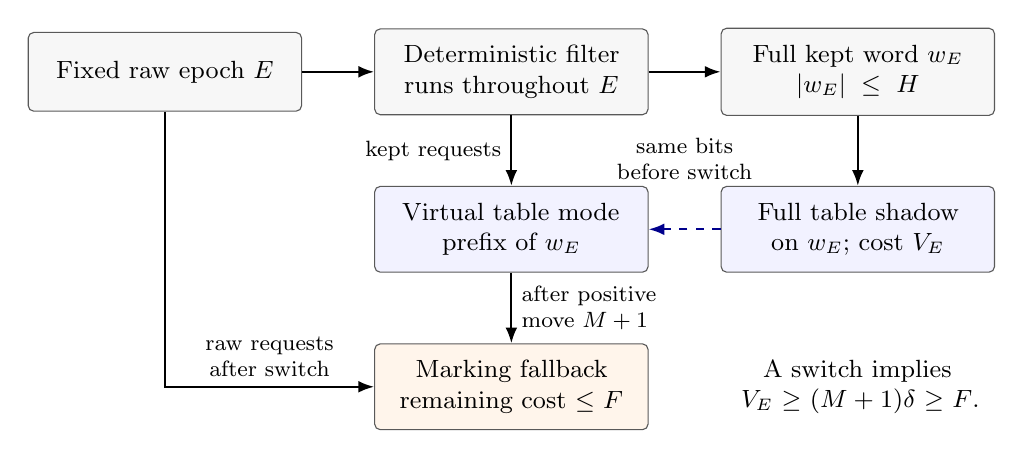
\begin{tikzpicture}[
  font=\small,
  box/.style={draw=black!65,rounded corners=2pt,align=center,
    inner sep=6pt,text width=3.05cm,minimum height=1.0cm},
  flow/.style={-{Latex[length=2mm]},thick},
  comparison/.style={flow,dashed,draw=blue!55!black}
]
\node[box,fill=black!3] (raw) at (0,0) {Fixed raw epoch $E$};
\node[box,fill=black!3] (filter) at (4.4,0)
  {Deterministic filter\\runs throughout $E$};
\node[box,fill=black!3] (word) at (8.8,0)
  {Full kept word $w_E$\\$|w_E|\le H$};
\node[box,fill=blue!5] (table) at (4.4,-2.0)
  {Virtual table mode\\prefix of $w_E$};
\node[box,fill=blue!5] (shadow) at (8.8,-2.0)
  {Full table shadow\\on $w_E$; cost $V_E$};
\node[box,fill=orange!8] (fallback) at (4.4,-4.0)
  {Marking fallback\\remaining cost $\le F$};
\node[align=center,text width=3.2cm] at (8.8,-4.0)
  {A switch implies\\$V_E\ge(M+1)\delta\ge F$.};
\draw[flow] (raw) -- (filter);
\draw[flow] (filter) -- (word);
\draw[flow] (filter) -- node[left,font=\footnotesize]{kept requests} (table);
\draw[flow] (word) -- (shadow);
\draw[comparison] (shadow) -- node[above=5mm,align=center,font=\footnotesize]
  {same bits\\before switch} (table);
\draw[flow] (table) -- node[right,align=left,font=\footnotesize]
  {after positive\\move $M+1$} (fallback);
\draw[flow] (raw.south) -- (0,-4.0) -- node[above,align=center,font=\footnotesize]
  {raw requests\\after switch} (fallback.west);
\end{tikzpicture}
\caption{The filter is independent of all sampled choices. The full shadow
is an analysis device on the deterministic word $w_E$; it continues after
the virtual service switches to fallback. Shared random bits identify the
table-mode prefix with a prefix of that shadow. Hence table-mode cost is at
most $V_E$, and a switch supplies another $V_E$ to pay for fallback.
The diagram shows data and comparison relations, not a common time scale.}
\label{fig:epoch-shadow}
\end{figure}


\begin{proposition}[Unbounded suffix guarantee]\label{prop:suffix}
For every fixed finite sequence $\sigma$, the routine starting at any
deterministic index, from arbitrary actual positions, has expected
suffix cost at most
\begin{equation}\label{eq:suffix-bound}
 (4a+2)\operatorname{OPT}_s(\sigma)+(2a+2)kD.
\end{equation}
Its table horizon and all parameters in
Equations~\eqref{eq:epoch-length}--\eqref{eq:suffix-parameters}
are fixed by the instance.
\end{proposition}

\begin{proof}
As observed when defining the blocks, the fixed whole-sequence optimum
pays at least $\delta$ inside each completed block, regardless of its
entering tuple. The completed blocks are disjoint intervals of request
times.

Let $N$ be the number of nonempty epochs.  The empty-suffix case is
immediate.  Otherwise the first $N-1$ epochs each contain $R$ completed
blocks, so
\[
 (N-1)R\delta\le \operatorname{OPT}_s(\sigma),
 \qquad
 N\le 1+\frac{\operatorname{OPT}_s(\sigma)}{kD},
\]
where $R\delta\ge kD$ follows from
Equation~\eqref{eq:epoch-length}.  Also
$\sum_E O_E\le\operatorname{OPT}_s(\sigma)$ because the epochs are
disjoint parts of the original sequence.  Summing
Equation~\eqref{eq:epoch-cost} therefore yields
\begin{align*}
 \E[\operatorname{cost}_{\rm suffix}]
 &\le 2a\operatorname{OPT}_s(\sigma)+(2a+2)kD\,N\\
 &\le (4a+2)\operatorname{OPT}_s(\sigma)+(2a+2)kD.
\end{align*}
\end{proof}

Only one epoch's fixed charge remains in this bound.  A final unfinished
epoch may contain arbitrarily many raw requests: its kept word is still
bounded by $H$, and its fallback cost is still bounded by $F$.  Thus no
table error or restart charge accumulates with the raw request count.

\section{A uniform schedule in the bit model}
\label{sec:uniform-computation}

The table and parameters of Section~\ref{sec:bounded-suffix} depend only on
the finite instance, but their construction need not be efficient.  We now
specify when that construction is performed and account for all computation
charged to an individual request.  The schedule uses the allowed dependence
on the binary length of the request counter.

\paragraph{Canonical preprocessing.}
Store $n,k,d$ in a fixed canonical encoding: binary integers have no leading
zeroes, each rational distance has a positive denominator and relatively
prime numerator and denominator, and matrix entries occur in their fixed
index order.  Use a fixed unambiguous encoding of lengths and delimiters.
Store the actual labeled tuple $s$, initialize a binary request counter to
zero, and initialize a flag indicating that suffix service has not started.
This takes a uniform polynomial number of bit operations in $L$ and produces
$O(L)$ bits.  For completeness, rational reduction is polynomial: long
division has polynomial bit cost, and in the Euclidean algorithm the larger
positive magnitude decreases by at least a factor of two within two
remainder steps.  Thus each reduction takes polynomially many bit
operations.  The explicit matrix encoding also gives $n\le O(L)$ and hence
$k\le O(L)$.  No table construction is part of preprocessing.

\paragraph{One finite constructor.}
Fix once and for all a deterministic, finite-alphabet bit machine $P$ with
the following behavior on the canonical encoding of $(n,k,d)$.  It computes
$D,\delta,R,F,M,H$, constructs the rational optimum and the dyadic table in
Proposition~\ref{prop:finite-table}, and writes its complete output on an
initially blank output tape.  It outputs the parameters, including $a$ and
$b$, and an explicit list of table records.  Each record contains its key
$(w,r,c)$ and the dyadic probability numerators in label order, with zero
numerators for disallowed labels.  Its strings and records are delimited
unambiguously.  Include, in addition, four unary strings of lengths
$H,R,M,b$.  If $S$ is the total output length in bits, then
\begin{equation}
 H,R,M,b\le S.
 \label{eq:unary-size}
\end{equation}
The output is a consecutively written finite string, so its representation
cannot describe a large blank or compressed table as though that table had
already been written.

All choices in $P$ are deterministic: use length and lexicographic orders
for finite indices and the fixed elimination, back-substitution, and
rounding rules from Section~\ref{sec:finite-tables}.  Exact integer and
rational operations are implemented by ordinary bit algorithms, rather
than counted as single machine steps.  Positivity of $\delta$ and
Proposition~\ref{prop:finite-table} show that $P$ halts on every valid
input.  Denote its finite number of elementary transitions by $T_P$, adding
an initial transition if necessary so that $T_P\ge1$.  Neither $C_0$, a
source policy, nor a bound on $T_P$ is an input to this machine.  In
particular, the existence theorem certifies feasibility of its finite
calculation; it supplies no computational oracle.

\begin{lemma}[Bounded implementation of the suffix]
\label{lem:bounded-implementation}
Given the explicitly written constructor output of length $S$, the suffix
routine can be implemented with a uniform polynomial number of bits of
storage and a uniform polynomial number of bit operations per request in
$L+S+2$.  These bounds hold for every reachable state and every outcome of
its random choices.  Each table sample uses exactly $b$ fresh unbiased
random bits.
\end{lemma}

\begin{proof}
Write $m=L+S+2$ for this proof.  By Equation~\eqref{eq:unary-size}, the numerical
values $H,R,M,b$ are at most $m$, and $n,k\le O(m)$.  Use explicit lists,
binary counters, and bounded strings for the following state.  The actual
and virtual tuples contain $k$ point indices each.  The kept word has at
most $H$ indices.  The filter has at most $H$ live entries by
Lemma~\ref{lem:filter}; each entry contains a tuple of $k$ indices and a
counter between zero and $M$.  Entries with the same data may remain
separate, as required by the filter construction.

For each raw request, scan every live tuple to determine whether it covers
that request.  If the request is kept, copy the surviving entries into a
new list and generate at most $k$ children for each removed entry.  Even an
implementation that temporarily materializes all $kH$ possible children
uses polynomial space: allowing $O(m)$ bits per index or counter gives
$O(m^3)$ bits for the old live list and $O(m^4)$ bits for all temporary
children.  Appending to the kept word and comparing or copying the lists
requires only polynomially many operations on those strings.  The final
list again has at most $H$ entries.  Continue these deterministic filter
updates in fallback mode as well, so the stored kept word is the whole
filtered prefix specified in Section~\ref{sec:bounded-suffix}.

The remaining state is also bounded.  Store the current raw block's set
of at most $k+1$ points, a counter of completed raw blocks bounded by
$R$, and the fallback marks together with their assigned labels.  Mark
sets have at most $k$ protected points; the possible next new point is
handled at that block's endpoint.  A mode flag and the virtual positive
move counter, capped at $M+1$, suffice for switching.  Set membership,
choice of the least eligible label, counter updates, and changes of tuple
entries all use finite scans and copies.  Epoch and block resets erase or
reuse precisely these bounded lists.  No raw epoch length, global epoch
number, cumulative movement total, or unfiltered request history is
stored.

At a table decision, locate the record by scanning the entire output and
comparing its key with the kept prefix, current request, and current
virtual tuple.  The key uses the prefix before appending the current kept
request.  Lemma~\ref{lem:filter} and the table-mode invariant ensure that
every required key has prefix length less than $H$.  All rows, including
rows whose original rational marginal was zero, were written by $P$.
Consequently lookup and the same storage bounds apply also to states
reached only through dyadic rounding.

If the row numerators are $N_1,\ldots,N_k$, draw exactly $b$ unbiased bits
to obtain a uniform integer $U\in\{0,\ldots,2^b-1\}$.  Choose the least
$j$ with $\sum_{i\le j}N_i>U$.  Such a $j$ exists because the numerators
sum to $2^b$; it is allowed because disallowed labels have numerator zero.
Only $k$ additions and comparisons of integers of at most $b+1$ bits are
needed, in addition to the $b$ random bits.  This sampling has no rejection
loop.  On a dropped table-mode request, or in fallback mode, the prescribed
label is found by the bounded scans already described.

These operations have a fixed number of nested loops, each over strings
or lists with polynomially bounded lengths.  Elementary arithmetic uses
bounded binary strings.  Implementing every access, scan, and copy on
ordinary tapes therefore gives a fixed-degree polynomial time bound, with
absolute constants. Use fixed-origin tape regions for the stored lists
and return their heads to those origins during cleanup.
At the end of each request discard or erase obsolete
lists and temporary strings, carrying only the stated compact state into
the next request.  Cleanup is included in the same polynomial bound.
Every bound is deterministic and independent of the probability of the
current state.
\end{proof}

\paragraph{The online schedule.}
At request number $t\ge1$, set
\begin{equation}
 g(t)=\lfloor\log_2(t+1)\rfloor.
 \label{eq:schedule-budget}
\end{equation}
Simulate $P$ from scratch on the stored canonical input for at most $g(t)$
elementary transitions.  If it has not halted, serve the current request
with label $1$.  If it has halted, use its output to serve the current
request by the suffix routine.  At the first successful simulation,
initialize a fresh suffix epoch, including this current request, and set
the activation flag.  At every later success, retain the suffix state
from the preceding request and perform its next step.  Recomputing the
identical table does not reset that state; only the prescribed epoch
boundaries do so.  Erase the simulation workspace and table after use,
preserving the canonical input, actual tuple, counter, activation flag,
and compact suffix state.

Figure~\ref{fig:activation} separates the repeated constructor simulation
from the persistent online state. The output-size estimate is the link
between the simulation budget and the suffix implementation bound.

\begin{proposition}[Uniform scheduling bound]
\label{prop:schedule}
There is one polynomial $p$, independent of the instance, such that
preprocessing uses at most $p(L)$ bit operations and serving request $t$
uses at most
\[
 p\bigl(L+\lceil\log_2(t+1)\rceil\bigr)
\]
bit operations, for every reachable history and internal state.  Activation
occurs at a finite deterministic time $t_*$ depending only on $(n,k,d)$.
\end{proposition}

\begin{proof}
The request counter has $O(g(t)+1)$ bits.  Incrementing it and determining
$g(t)$ costs a polynomial in its length.  A simulation lasting at most
$g(t)$ elementary transitions uses the copied input and at most
$O(g(t)+1)$ additional cells on each of a fixed number of tapes.  Explicit
tape simulation, including copying the $O(L)$-bit input, locating tape
heads, counting transitions, and erasing the workspace, has uniform
polynomial cost in $L+g(t)+2$.  This assertion concerns the actual capped
simulation; it does not charge an uncapped arithmetic subroutine as one
transition.

Whenever a simulation succeeds, a fixed finite-alphabet machine has
written at most a constant times $g(t)+1$ output bits.  Thus
\begin{equation}
 S=O(g(t)+1)
 \label{eq:output-budget}
\end{equation}
before any suffix operation is attempted.  Lemma~\ref{lem:bounded-implementation}
then bounds all suffix work by a uniform polynomial in $L+g(t)+2$.
The failure action, updating the actual tuple, and issuing the chosen
label have smaller polynomial bounds.  The preceding request's budget
was no larger than the current one.  Its compact state and any storage
to be accessed, copied, or erased are consequently bounded by the same
current polynomial.  Our cleanup convention leaves no accumulated
workspace depending on the number of earlier requests.  This also
accounts for the first initialization and every later reset.

Choose absolute constants $A$ and an integer $c$ large enough to dominate
these finitely many polynomial bounds, and set $p(x)=A(x+2)^c$.  Increase
$A,c$ if necessary to cover preprocessing.  Since
$g(t)\le\lceil\log_2(t+1)\rceil$, this is the single polynomial asserted.
The bound is worst case, so it implies the required conditional expected
bound at every reachable state.

Finally, define for analysis only
\begin{equation}
 t_* = \min\{t\ge1:g(t)\ge T_P\}=2^{T_P}-1.
 \label{eq:activation-time}
\end{equation}
It is finite.  The constructor and its canonical input depend only on
$(n,k,d)$, so the same is true of $T_P$ and $t_*$.  In particular,
irrelevant padding or unreduced representations of the original rational
input cannot change this threshold, nor can $s$ or the request sequence.
Monotonicity of $g$ ensures that every simulation from $t_*$ onward
succeeds.  The algorithm never computes $T_P$ or $t_*$ in advance; it
detects success by the ordinary halting state of its capped simulation.
\end{proof}

\begin{figure}[tbp]
\centering
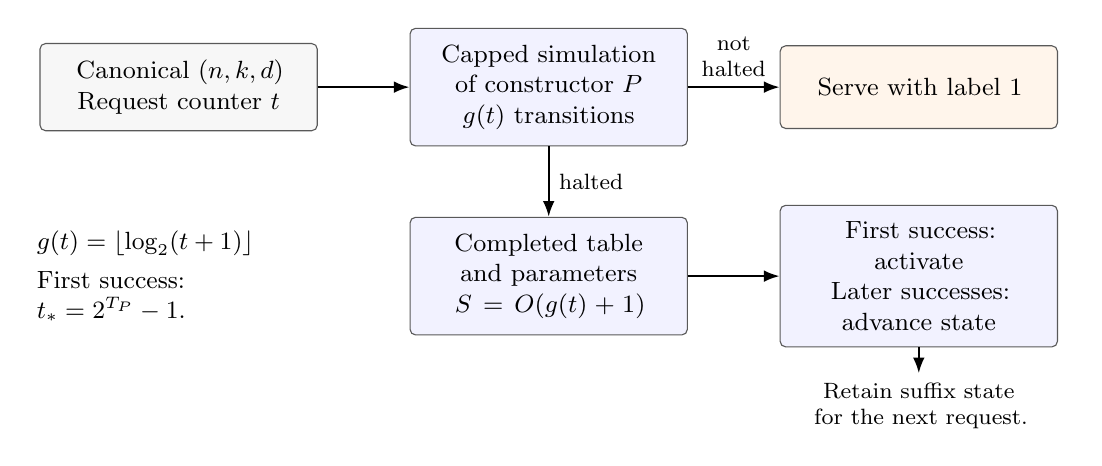
\begin{tikzpicture}[
  font=\small,
  box/.style={draw=black!65,rounded corners=2pt,align=center,
    inner sep=6pt,text width=3.1cm,minimum height=1.05cm},
  flow/.style={-{Latex[length=2mm]},thick}
]
\node[box,fill=black!3] (input) at (0,0)
  {Canonical $(n,k,d)$\\Request counter $t$};
\node[box,fill=blue!5] (simulate) at (4.7,0)
  {Capped simulation\\of constructor $P$\\$g(t)$ transitions};
\node[box,fill=orange!8] (failure) at (9.4,0)
  {Serve with label $1$};
\node[box,fill=blue!5] (output) at (4.7,-2.4)
  {Completed table\\and parameters\\$S=O(g(t)+1)$};
\node[box,fill=blue!5] (suffix) at (9.4,-2.4)
  {First success:\\activate\\Later successes:\\advance state};
\node[align=center,text width=3.7cm,font=\footnotesize] (state) at (9.4,-4.05)
  {Retain suffix state\\for the next request.};
\node[align=left,text width=3.6cm] at (0,-2.4)
  {$g(t)=\lfloor\log_2(t+1)\rfloor$\smallskip\\
   First success:\\$t_*=2^{T_P}-1$.};
\draw[flow] (input) -- (simulate);
\draw[flow] (simulate) -- node[above,align=center,font=\footnotesize]{not\\halted} (failure);
\draw[flow] (simulate) -- node[right,font=\footnotesize]{halted} (output);
\draw[flow] (output) -- (suffix);
\draw[flow] (suffix.south) -- (state.north);
\end{tikzpicture}
\caption{Each request pays for a fresh capped simulation. Before activation,
only one fixed label serves requests. After activation, the complete table's
explicit size fits the current budget, and the suffix routine advances its
persistent state, with resets only at its prescribed epoch boundaries.
The construction time $T_P$ and activation time $t_*$ are
finite instance-dependent quantities; their magnitude enters the additive
movement term.}
\label{fig:activation}
\end{figure}


\begin{proof}[Proof of Theorem~\ref{thm:main}]
The preprocessing and online schedule above define a uniform causal
algorithm using only unbiased random bits.  Every decision serves the
current request by moving one labeled actual server.  By
Proposition~\ref{prop:schedule}, its bit complexity has the required bound
with one polynomial $p$.

Fix any finite request sequence $\sigma$ independent of the random bits.
The requests before activation cost at most
$(t_*-1)D$ in total, since each moves a single server over distance at most
$D$.  If $\sigma$ ends before activation, this already bounds its entire
cost.  Otherwise Proposition~\ref{prop:suffix}, applied to the suffix
starting at the deterministic time $t_*$ and compared with the optimum
from $s$ for the whole sequence, gives
\begin{equation}
 \E[\operatorname{cost}_A(\sigma)]
 \le (4a+2)\operatorname{OPT}_s(\sigma)
       +(t_*-1)D+(2a+2)kD.
 \label{eq:full-movement-bound}
\end{equation}
The same inequality holds for shorter sequences, including the empty
sequence, by nonnegativity of its right-hand terms.

Since $a\le C_0\log^2(k+1)$ and $\log(k+1)\ge\log3$, set
\begin{equation}
 C=4C_0+\frac{2}{(\log3)^2},
 \qquad
 B_{d,k,s}=(t_*-1)D+(2a+2)kD.
 \label{eq:final-constants}
\end{equation}
Then $4a+2\le C\log^2(k+1)$, proving the desired movement inequality.
The constant $C$ is absolute, and $B_{d,k,s}$ is finite and depends only
on the instance.  Its formula happens not to require $s$.  Repeated
positions in $s$ cause no difficulty: the suffix comparison allowed
arbitrary actual starting tuples, while the existence theorem and finite
table were used only from the distinct virtual tuple $u$.
\end{proof}

\section{Scope of the construction}\label{sec:conclusion}

The construction converts the companion existence theorem into one uniform
algorithm on finite rational metrics. The policy guaranteed there is never
executed or queried: it certifies feasibility of the finite flow system.
A rational solution is computed, and its conditional rows are rounded to
dyadic probabilities before sampling with unbiased bits. The
deterministic filter makes a single finite table sufficient for arbitrarily
long epochs, without a rounding loss proportional to their raw length.

The computational guarantee rests on the permitted dependence on the
binary request-counter length. The constructor's running time $T_P$ gives
activation time $2^{T_P}-1$, and the movement before activation enters the
additive constant in Equation~\eqref{eq:final-constants}. These quantities
are finite, with no useful size bound asserted here. The construction
leaves open the same ratio with a useful bound on startup movement or with
a uniform polynomial per-request bound in $L$ alone.

\bibliographystyle{plain}
\bibliography{references}
\end{document}
